%% needed for the template to find the class dir when the class folder
%% is not stored in the same directory than the main tex file
\def\classdir{dibiso} % TODO: fix undefined classdir + improved explanations

\newcommand{\reportyear}{2024}
\newcommand{\halcollectionid}{UNIV-PARIS-SACLAY}
\newcommand{\labacronym}{UPSaclay}
\newcommand{\labfullname}{Université Paris-Saclay}
\newcommand{\datafetchdate}{24/09/2025}
\newcommand{\watermarktext}{}

\newcommand{\anrprojectsinfo}{Le nombre d'entités affichées a été limité à 20. Dans l'API, 1637 entités ont été trouvées.\\}
\newcommand{\chaptersinfo}{}
\newcommand{\collaborationsnb}{2957}
\newcommand{\institutionsnb}{1269}
\newcommand{\countriesnb}{82}
\newcommand{\collaborationmapworldinfo}{\emoji{warning} Le traitement des données a été limité par le nombre maximal d'entités téléchargeables (1000). Des données peuvent être manquantes ou les valeurs peuvent être inférieures aux valeurs réelles. \\}
\newcommand{\collaborationmapeuropeinfo}{\emoji{warning} Le traitement des données a été limité par le nombre maximal d'entités téléchargeables (1000). Des données peuvent être manquantes ou les valeurs peuvent être inférieures aux valeurs réelles. \\}
\newcommand{\collaborationnamesinfo}{Le nombre d'entités affichées a été limité à 40. Dans l'API, 14322 entités ont été trouvées.\\}
\newcommand{\conferencesinfo}{Le nombre d'entités affichées a été limité à 40. Dans l'API, 2609 entités ont été trouvées.\\}
\newcommand{\europeanprojectsinfo}{Le nombre d'entités affichées a été limité à 20. Dans l'API, 551 entités ont été trouvées.\\}
\newcommand{\bsojournalsnbworks}{1000}
\newcommand{\bsojournalsnbworksfoundinbso}{792}
\newcommand{\bsojournalsnbjournals}{503}
\newcommand{\bsojournalsbsoversion}{2024Q4}
\newcommand{\journalsinfo}{\emoji{warning} Le traitement des données a été limité par le nombre maximal d'entités téléchargeables (1000). Des données peuvent être manquantes ou les valeurs peuvent être inférieures aux valeurs réelles. \\}
\newcommand{\journalshalinfo}{Le nombre d'entités affichées a été limité à 40. Dans l'API, 3407 entités ont été trouvées.\\}
\newcommand{\oaworksperiod}{2020 - 2024}
\newcommand{\openaccessworksinfo}{}
\newcommand{\privatesectorcollaborationsinfo}{\emoji{warning} Le traitement des données a été limité par le nombre maximal d'entités téléchargeables (1000). Des données peuvent être manquantes ou les valeurs peuvent être inférieures aux valeurs réelles. \\}
\newcommand{\workstypeinfo}{}



\documentclass[french, 11pt]{dibiso/biso}

\title{Bilan \\ Science \\ Ouverte}

\author{Direction des bibliothèques, de l’information et de la science ouverte}

\date{Année \reportyear}

\subtitle{\textbf{Laboratoire \labacronym} \\
  \medskip
  \labfullname
}

% Remplacez Reporter Name par votre nom :
\reporter{Reporter Name}
% Remplacez reporter.email@example.com par votre email :
\reporteremail{reporter.email@example.com}


%%%%%%%%%%%%%%%%%%%%%%%%%%% COMMENT REMPLIR LE BISO %%%%%%%%%%%%%%%%%%%%%%%%%%%
%                                                                             %
% Commenter des parties à exclure :                                           %
% Pour commenter des sections que vous ne souhaitez pas inclure dans le       %
% rapport final, vous pouvez utiliser le symbole % au début de chaque ligne   %
% que vous souhaitez exclure. Cela peut vous servir à ne pas afficher des     %
% sections du rapports que vous ne jugez pas appropriées pour le laboratoire. %
%                                                                             %
%                                                                             %
% Créer une liste à puces :                                                   %
% Pour créer une liste à puces, utilisez l'environnement itemize. Voici un    %
% exemple :                                                                   %
% \begin{itemize}                                                             %
%     \item Premier élément de la liste                                       %
%     \item Deuxième élément de la liste                                      %
%     \item Troisième élément de la liste                                     %
% \end{itemize}                                                               %
%                                                                             %
%                                                                             % 
% Mettre du texte en gras :                                                   %
% Pour mettre du texte en gras, utilisez la commande \textbf{}. Par exemple : %
% Voici un exemple de \textbf{texte en gras}.                                 %
%                                                                             %
%%%%%%%%%%%%%%%%%%%%%%%%%%% COMMENT REMPLIR LE BISO %%%%%%%%%%%%%%%%%%%%%%%%%%%


\begin{document}

\renewcommand{\arraystretch}{1.5}


\maketitle

\tableofcontents

\pagebreak



\section{Introduction}


\subsection*{Méthodologie et objectifs }

Le BISO est un bilan science ouverte établi sur les publications déposées dans HAL. Il est produit à l’automne afin de permettre une plus grande exhaustivité des dépôts référencés dans la collection HAL du laboratoire. 


\subsection*{Calendrier annuel }

\begin{enumerate}
  \item Printemps : Le 3RSO envoie une liste des publications manquantes dans HAL au DU du laboratoire.
  \item Été : les chercheurs et doctorants sont invités à déposer les publications manquantes dans HAL, idéalement en déposant le texte intégral (version postprint) ou à défaut les notices bibliographiques.
  \item Automne : votre référent recherche produit le BISO et le communique à la directrice, directeur de laboratoire.
\end{enumerate}


Ce bilan est proposé pour donner un aperçu annuel des atouts SO du laboratoire, en présentant une liste exhaustive des revues, conférences, et collaborations, accompagné d’un relevé des actions en faveur de la science ouverte, et de propositions d’amélioration.

Ce document est à l’attention des directeurs, directrices, et toute personne du laboratoire qui participe activement aux actions de développement de la Science Ouverte. Communiqué seulement en interne, il permet aux référents recherche de vous présenter des données HAL, préalablement nettoyées, avec la participation des chercheurs pour les dépôts, afin de refléter au mieux la production scientifique. Remis chaque année,  le BISO vise également à vous aider à anticiper la préparation de rapports (ex : HCERES).


% Ecrire l'introduction ci-dessous :



% Fin de l'introduction

\pagebreak

\section{Liste des revues}

A partir des publications déposées dans HAL, liste des revues dans le Baromètre de la Science Ouverte.

TOTO: add figure
%{
%  \footnotesize
%  \begin{longtable}{p{.55\linewidth}P{.08\linewidth}P{.11\linewidth}P{.11\linewidth}}
\caption{Liste des revues}
\label{tab_journals}\\
\toprule
Revue & Nombre de publications & Status des accès ouverts des publications & APC payés \\
\midrule
Volume 3A: Combustion, Fuels, and Emissions & \makecell{3} & \makecell{2 closed, \\ 1 green} & \makecell{} \\
Proceedings of the Combustion Institute & \makecell{7} & \makecell{6 other, \\ 1 hybrid} & \makecell{2 980 USD} \\
International Journal of Heat and Mass Transfer & \makecell{1} & \makecell{1 other} & \makecell{} \\
Chemical Engineering Research and Design & \makecell{2} & \makecell{2 green} & \makecell{} \\
Combustion and Flame & \makecell{4} & \makecell{4 other} & \makecell{} \\
Volume 3B: Combustion, Fuels, and Emissions & \makecell{1} & \makecell{1 green} & \makecell{} \\
Plasma Sources Science and Technology & \makecell{4} & \makecell{2 closed, \\ 2 green} & \makecell{} \\
Journal of Engineering for Gas Turbines and Power & \makecell{3} & \makecell{2 closed, \\ 1 green} & \makecell{} \\
Aerospace & \makecell{1} & \makecell{1 gold} & \makecell{1 600 CHF} \\
Applications in Energy and Combustion Science & \makecell{4} & \makecell{4 gold} & \makecell{2 000 USD, \\ 2 000 USD, \\ 2 000 USD, \\ 2 000 USD} \\
AIAA Journal & \makecell{1} & \makecell{1 green} & \makecell{} \\
Applied Physics B & \makecell{3} & \makecell{3 green} & \makecell{} \\
AIAA SCITECH 2023 Forum & \makecell{1} & \makecell{1 green} & \makecell{} \\
Computers \& Fluids & \makecell{1} & \makecell{1 green} & \makecell{} \\
International Journal of Multiphase Flow & \makecell{1} & \makecell{1 closed} & \makecell{} \\
CEAS Space Journal & \makecell{1} & \makecell{1 green} & \makecell{} \\
Frontiers in Physics & \makecell{1} & \makecell{1 gold} & \makecell{2 490 USD} \\
Biophysical Journal & \makecell{1} & \makecell{1 hybrid} & \makecell{2 500 USD} \\
Journal of Thermophysics and Heat Transfer & \makecell{1} & \makecell{1 green} & \makecell{} \\
Journal of Aerosol Science & \makecell{1} & \makecell{1 green} & \makecell{} \\
International Journal of Thermal Sciences & \makecell{1} & \makecell{1 green} & \makecell{} \\
Proceeding of International Heat Transfer Conference 17 & \makecell{1} & \makecell{1 green} & \makecell{} \\
\bottomrule
\end{longtable}

%}

% Ecrire un commentaire sur la liste des revues ci-dessous :





% Fin de la liste des revues

\pagebreak

\section{Liste des conférences}

\begin{figure}[!h]
  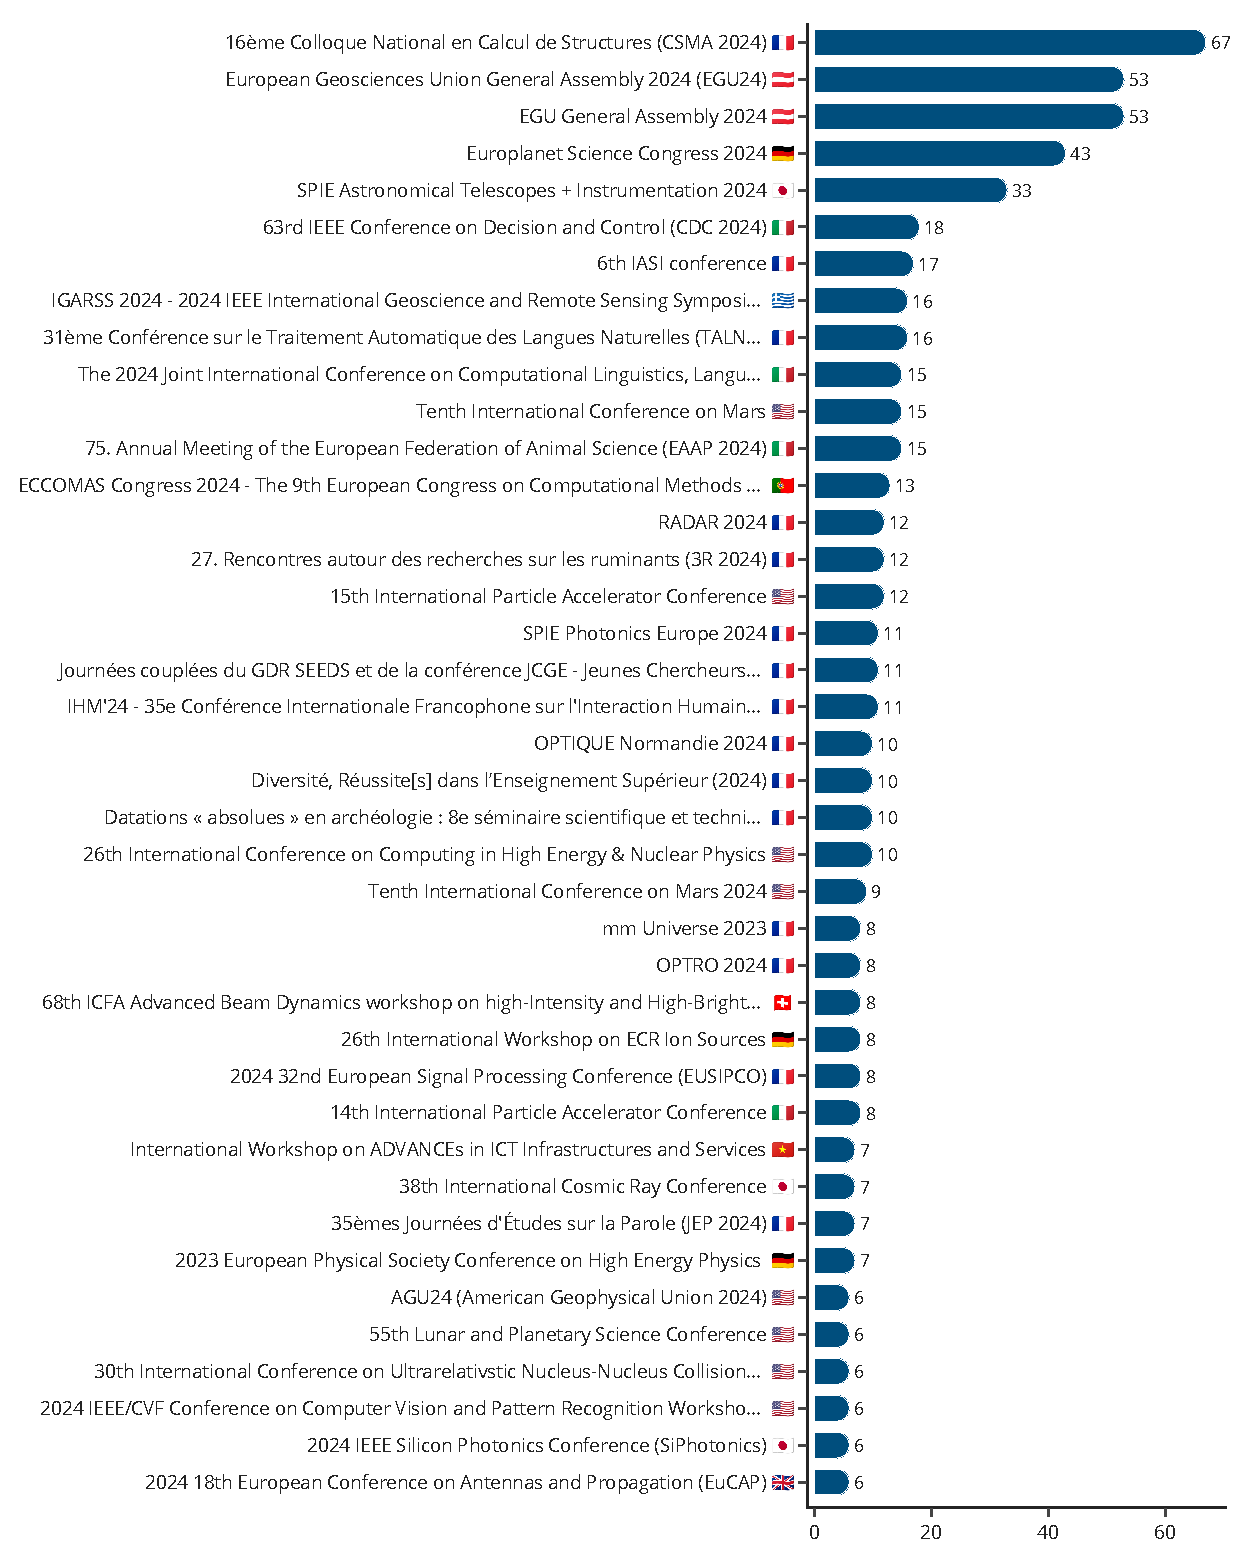
\includegraphics[width=\textwidth]{figures/conferences.pdf}
  \centering
  \caption{Conférences}
  \label{fig_conferences}
\end{figure}

% Ecrire un commentaire sur la liste des conférences ci-dessous :





% Fin de la liste des conférences


\pagebreak

\section{Liste des chapitres}

{
  \footnotesize
  \begin{longtable}{p{.4\linewidth}p{.35\linewidth}p{.15\linewidth}}
\caption{Liste des chapitres renseignés dans HAL}
\label{tab_chapters}\\
\toprule
Titre du chapitre & Titre du livre & Éditeur \\
\midrule
L'agriculture a-t-elle sa place en ville ? & "Ressources" n°6, la revue INRAE &  \\
Die Medien: Schlachten der Kommunikation & Springer eBooks &  \\
Under the ICSU Umbrella: The Joint Commission on Radioactivity (1947-1955) between IUPAP and IUPAC & Globalizing Physics. One Hundred Years of the International Union of Pure and Applied Physics & Oxford University Press \\
Struggles Over the Definition of a “Job Well Done” & Encyclopedia of Professionalization: Organization of Professions, Production of Professionalities and Growth of Professionalism & Wiley \\
Scientific workflows management with blockchain: a survey & Blockchain and smart-contract technologies for innovative applications & Springer Cham \\
Guerre froide : Relations avec des physiciens soviétiques & Les sciences en guerre froide (1946-1991) — France — Union soviétique et pays de l'Est — Témoignages - (coordinateur Claude Debru) & Presses universitaires Rhin \& Danube \\
Some réminiscences & Les sciences en guerre froide (coordinateur: Claude Debru) &  \\
Metallo-β-lactamases & Metalloenzymes & Elsevier \\
L'économie sociale et solidaire : antitode ou excipient du néolibéralisme ? Quelques réflexions à partir du monde associatif & (Re)penser l'économie sociale et solidaire. Approches et historiographie & L'Arbre bleu \\
Transformations de la fonction RH & Ressources Humaines - 4ème édition & Dunod \\
Du dancing à la scène : le jazz dans les casinos de Vichy & Martin Guerpin et Etienne Jardin (dir.) Faites vos jeux ! La vie musicale dans les casinos français (19e-21e siècle) &  \\
Entre Alger et Lunéville. Récits de santé d’une famille bourgeoise & L’orientalisme en train de se faire & EHESS \\
« Les reconversions empêchées des ex-salariés de Renault Billancourt », in Emmanuel de Lescure, Nicolas Divert, Fabienne Maillard, , Rennes, Presses Universitaires de Rennes, 2024. & La formation continue au service de la reconversion ? Les liens fragiles entre aspirations et mobilités dans le monde du travail &  \\
ICT externalities: measurement issues and their effects on output growth & Intangible assets, productivity and economic growth : micro, meso and macro perspectives & Routledge \\
A Conference For Africa. Racialization and the New World Order & The Paris Peace Conference of 1919: The Challenge of a New World Order & Berghahn Books \\
Les frères Basset ou les voies diverses de la colonisation & L’orientalisme en train de se faire & EHESS \\
Les modèles constitutionnels anglais et américain dans l’historiographie constitutionnelle comparée du XIXe siècle & Historiographies constitutionnelles et identités nationales (sous la coordination de Jacky Hummel) & Mare \& Martin \\
Conseil constitutionnel, 14 avril 2023, n° 2023-849, Loi de financement de la sécurité sociale pour 2023 & Les grandes décisions de la jurisprudence constitutionnelle. Approche politique & LGDJ \\
Le nouveau service de l'Etat. Sociologie des régulateurs français & Le moment régulateur. Naissance d'une contre-culture de gouvernement & Presses de Sciences Po \\
Semiparametric estimation in elliptical distributions & Elliptically Symmetric Distributions in Signal Processing and Machine Learning &  \\
Physics-based output-feedback consensus-formation control of networked autonomous vehicles & Hybrid and Networked Dynamical Systems & Springer Verlag \\
Introduction générale : Faire des finances syndicales un objet de recherche & Les finances syndicales & Septentrion \\
L'anthropologie des historiens & Histinéraires. La fabrique de l’histoire telle qu’elle se raconte. Une enquête sur les historiens contemporains &  \\
Ouvertures & Enquêter sur ce qui se passe. Mélanges offerts à Antoine Hennion & Presses des Mines \\
Des inégalités et injustices climatiques à la transition juste ? & Les sociétés face aux défis climatiques : que sait-on ? & CNRS Editions \\
\textbf{Seulement 25 lignes affichées sur 496.} \\
\bottomrule
\end{longtable}

}

% Ecrire un commentaire sur la liste des chapitres ci-dessous :





% Fin de la liste des chapitres

\pagebreak

\section{Typologie de la production scientifique}

\begin{figure}[!h]
  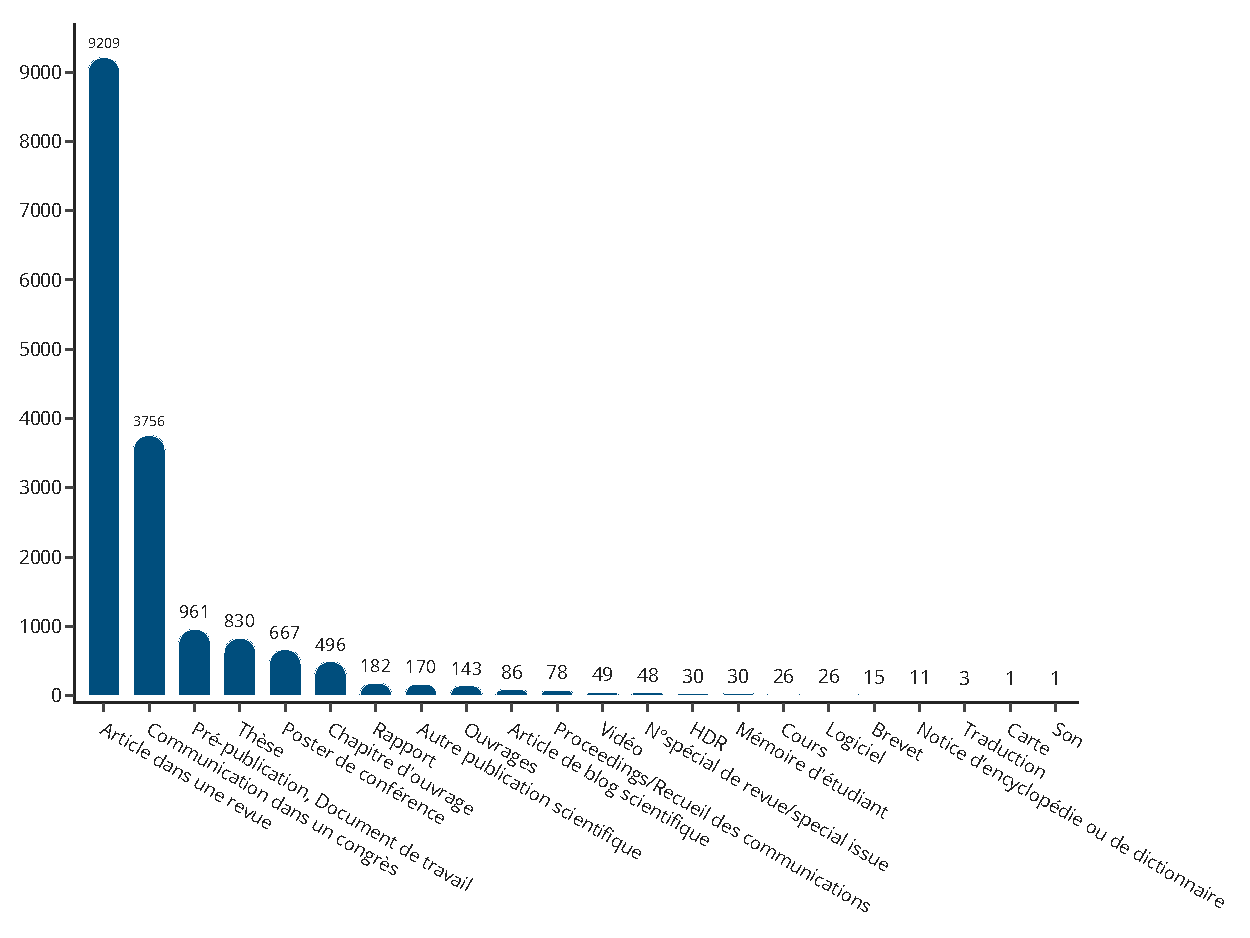
\includegraphics[width=\textwidth]{figures/works_type.pdf}
  \centering
  \caption{Types de documents}
  \label{fig_doc_type}
\end{figure}

% Ecrire un commentaire sur la typologie de la production scientifique ci-dessous :





% Fin de la typologie de la production scientifique

\pagebreak

\section{Articles et Communications de congrès en accès libre} % Evolution sur une période de 5 ans (2020-2024)

\begin{figure}[!h]
  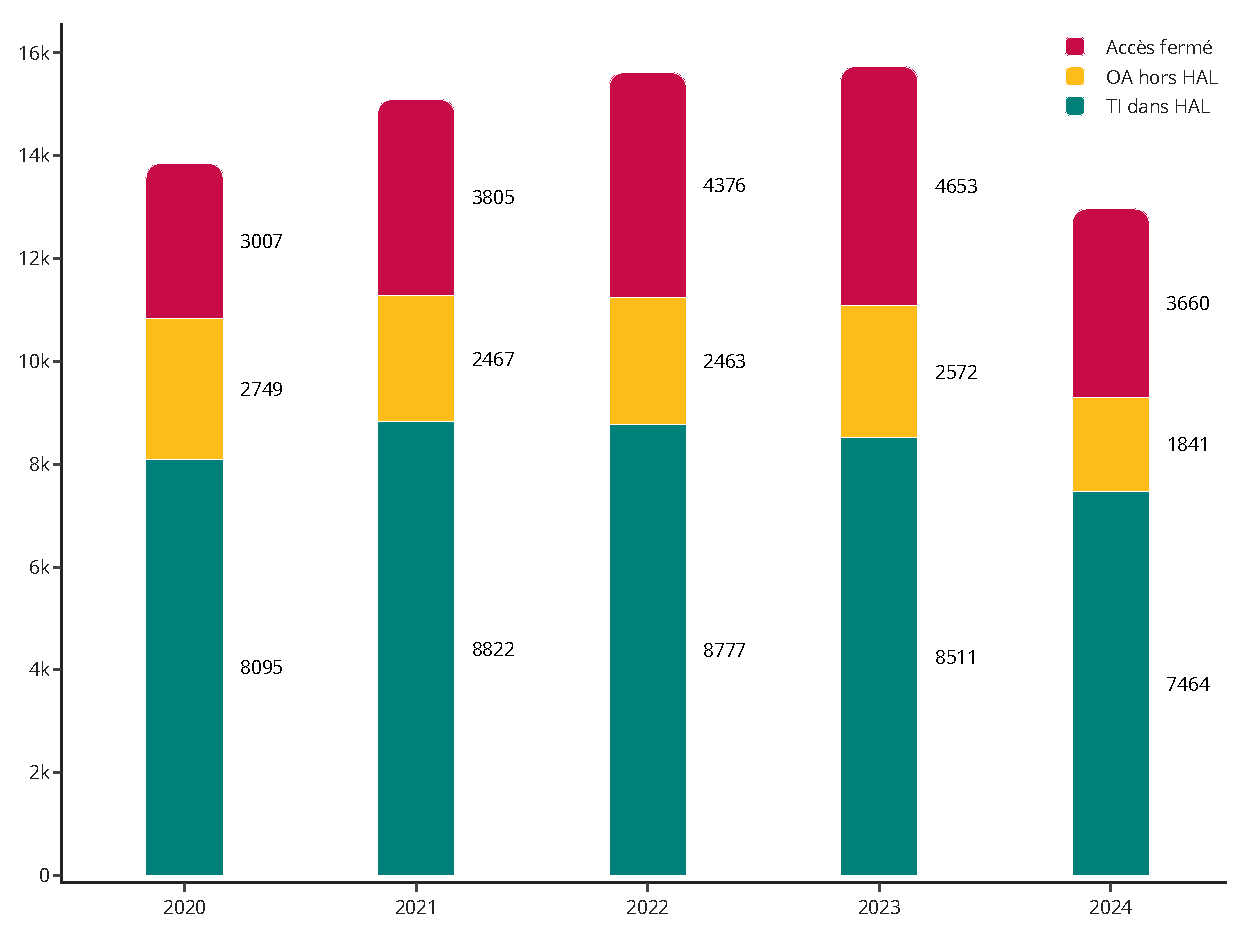
\includegraphics[width=\textwidth]{figures/open_access_works.pdf}
  \caption{Statut des accès ouverts des travaux sur la période {\oaworksperiod}}
  \label{fig_open_access_works}
\end{figure}

% Ecrire un commentaire sur les articles et communication de congrès en accès libre ci-dessous :





% Fin des articles et communication de congrès en accès libre

\pagebreak

\section{Carte des collaborations internationales}

{\collaborationsnb} collaborations parmi {\institutionsnb} institutions dans {\countriesnb} pays d'après la liste des articles avec un DOI dans HAL et les données de collaboration d'OpenAlex.

\begin{figure}[!h]
  \hspace{-.1\textwidth}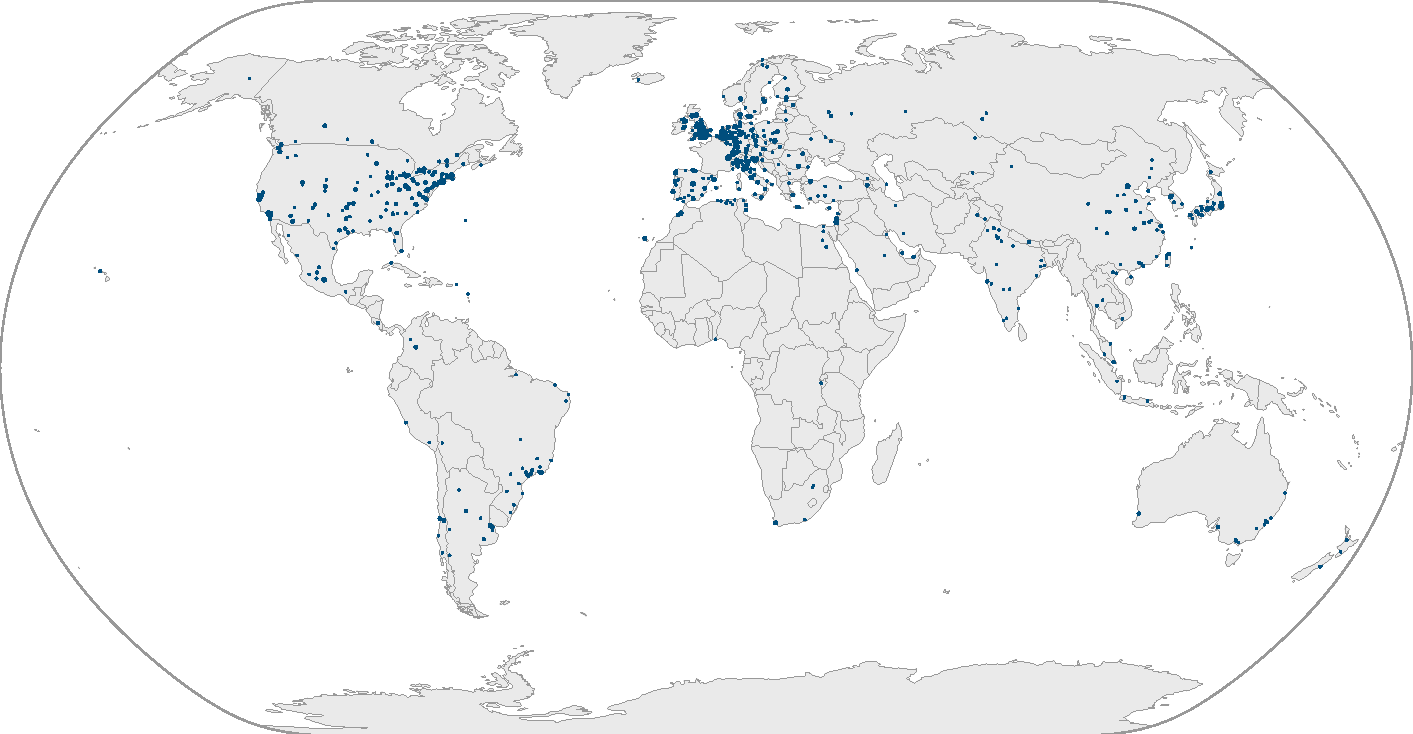
\includegraphics[width=1.2\textwidth]{figures/collaboration_map_world.pdf}
  \caption{Collaborations internationales hors France - Données : publications renseignées dans HAL avec un DOI, en utilisant les métadonnées d'OpenAlex}
  \label{fig_collab_map}
\end{figure}

% Ecrire un commentaire sur la carte des collaborations internationales ci-dessous :





% Fin de la carte des collaborations internationales

\pagebreak

\section{Carte des collaborations Européennes}

\begin{figure}[!h]
  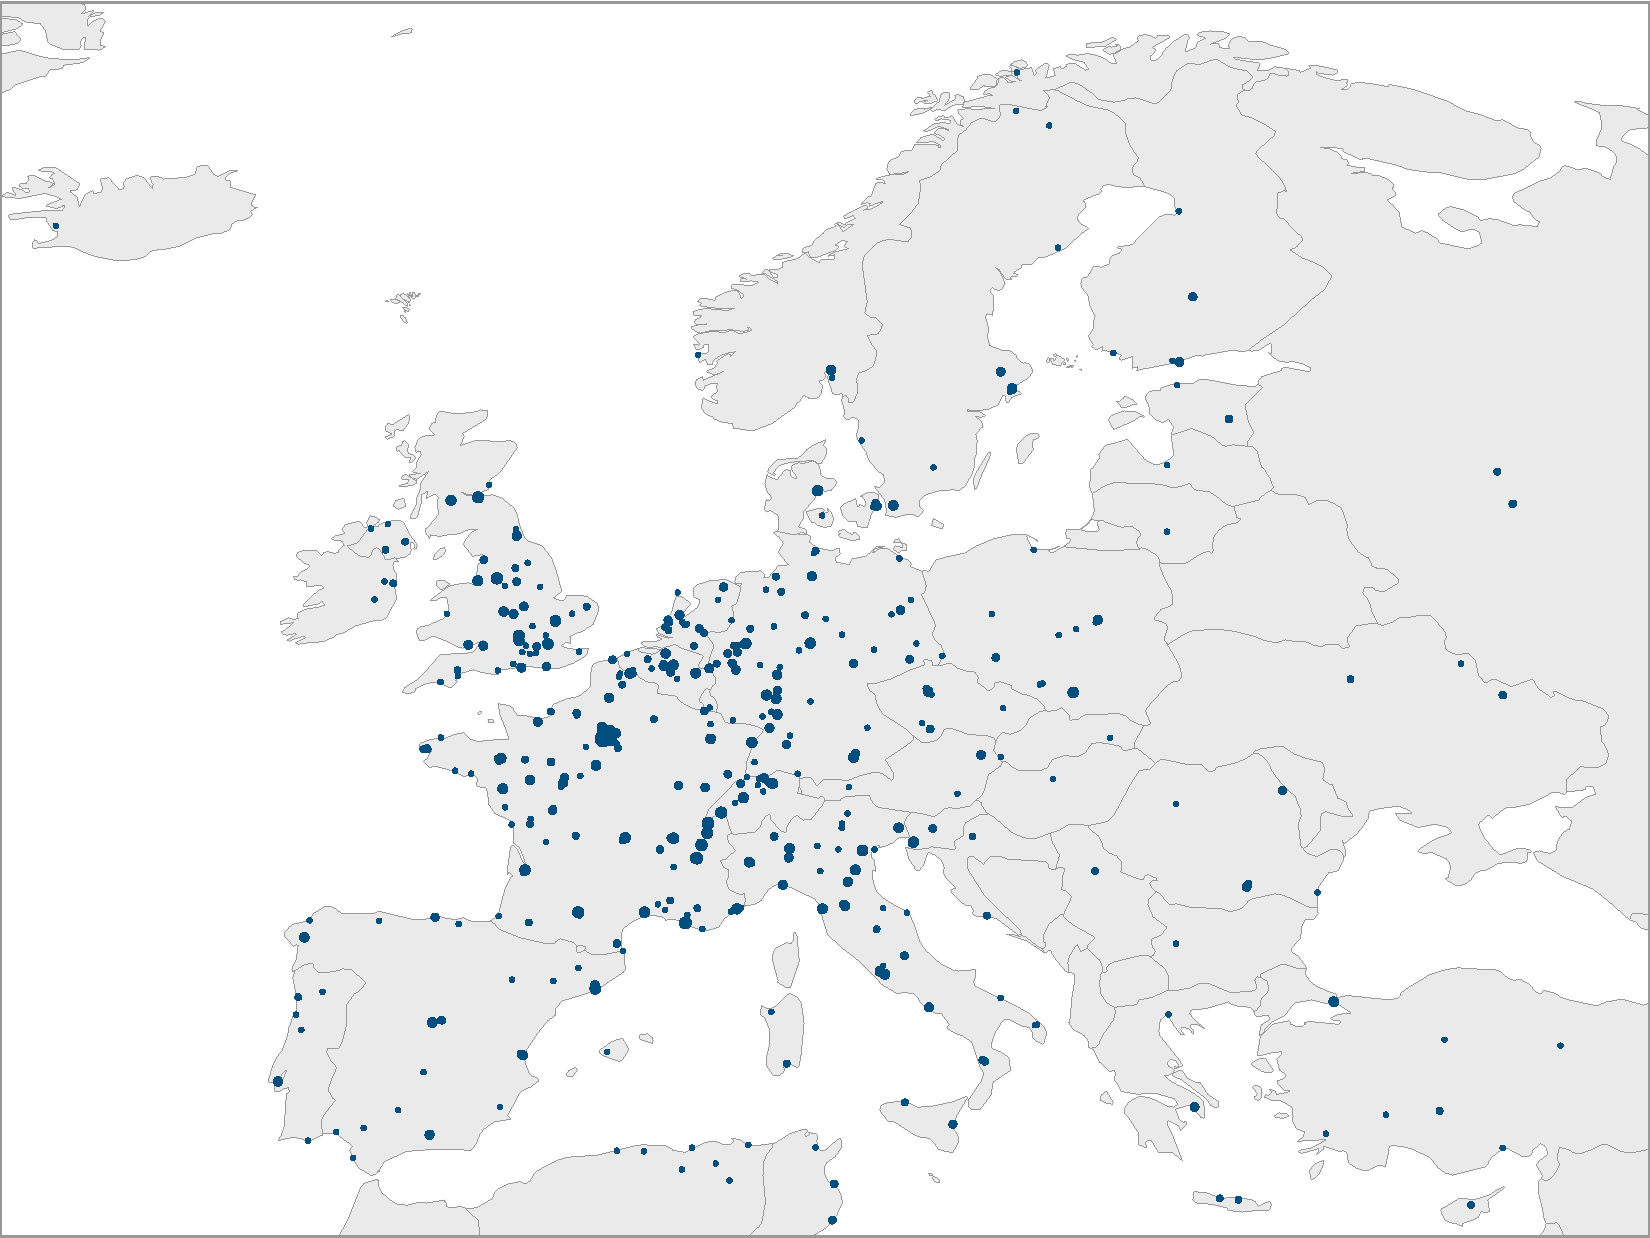
\includegraphics[width=\textwidth]{figures/collaboration_map_europe.pdf}
  \caption{Collaborations Européennes - Données : publications renseignées dans HAL avec un DOI, en utilisant les métadonnées d'OpenAlex}
  \label{fig_collab_map_europe}
\end{figure}

% Ecrire un commentaire sur la carte des collaborations Européennes ci-dessous :





% Fin de la carte des collaborations Européennes

\pagebreak

\section{Collaborations internationales par établissements}

\begin{figure}[!h]
  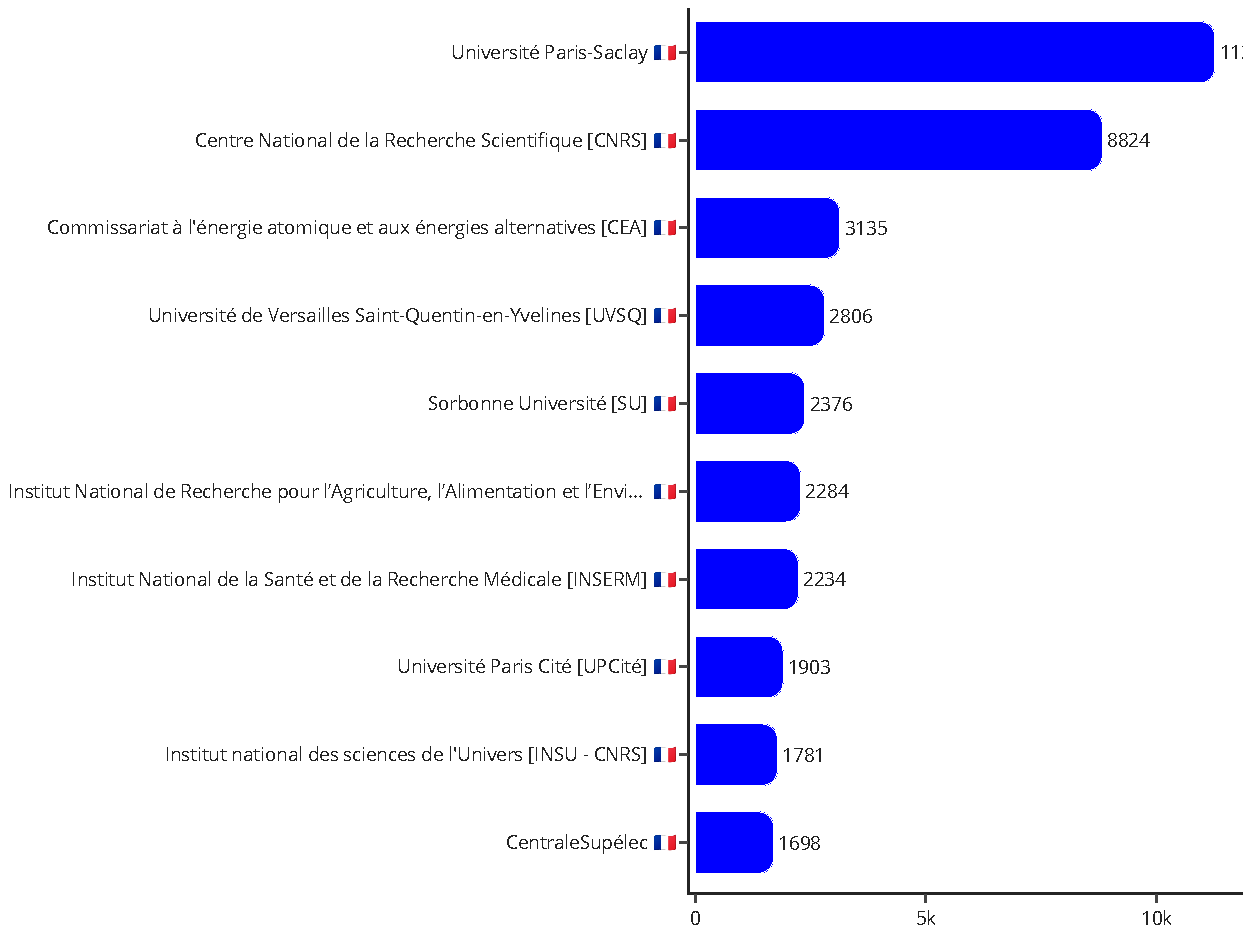
\includegraphics[width=\textwidth]{figures/collaboration_names.pdf}
  \caption{Collaborations internationales hors France - Données : Nom des institutions renseignées dans HAL}
  \label{fig_collab_names}
\end{figure}

% Ecrire un commentaire sur les collaborations internationales par établissements ci-dessous :





% Fin des collaborations internationales par établissements

\pagebreak

\section{Collaborations (non académique) avec le secteur privé}

TODO: add figure

% Ecrire un commentaire sur les collaborations (non académique) avec le secteur privé  ci-dessous :





% Fin des collaborations (non académique) avec le secteur privé

\pagebreak

\section{Publications liées à des projets européens}

\begin{figure}[!h]
  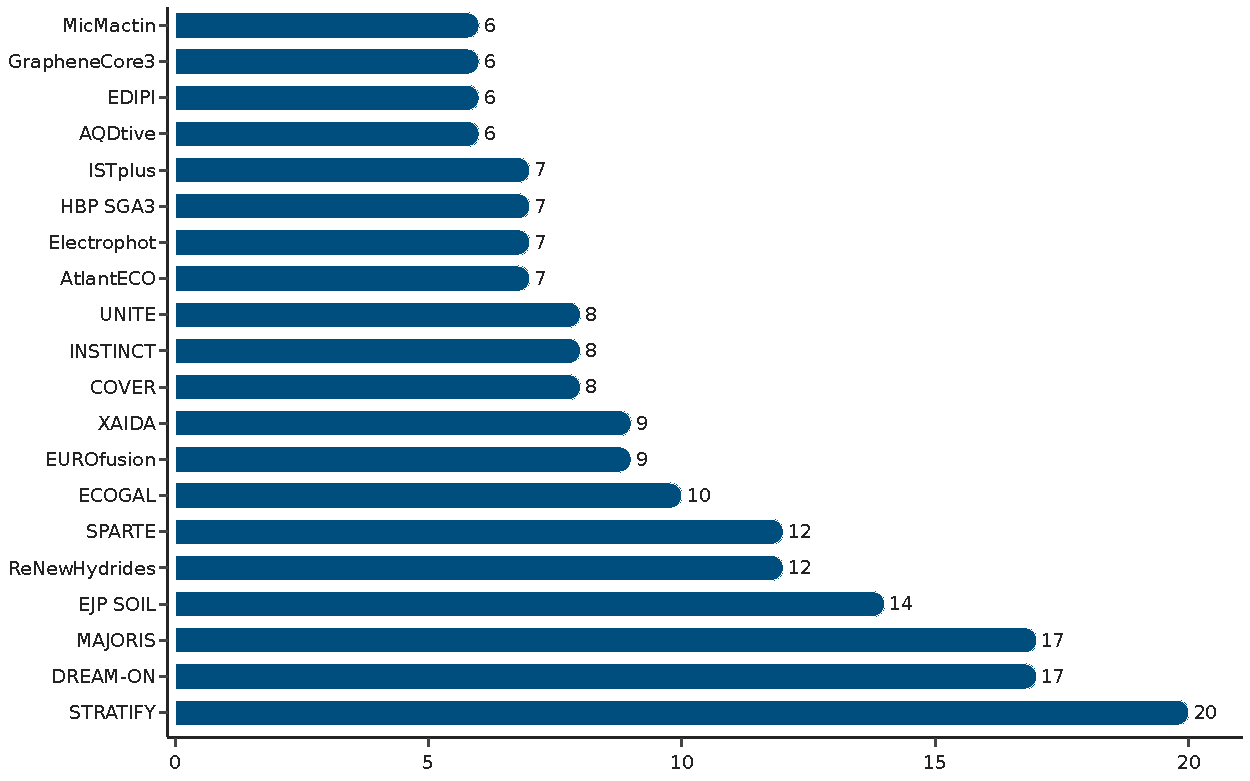
\includegraphics[width=.8\textwidth]{figures/european_projects.pdf}
  \centering
  \caption{Projets Européens}
  \label{fig_eu_projects}
\end{figure}

% Ecrire un commentaire sur les publications liées à des projets européens ci-dessous :





% Fin des publications liées à des projets européens


\section{Publications liées à des projets ANR}

\begin{figure}[!h]
  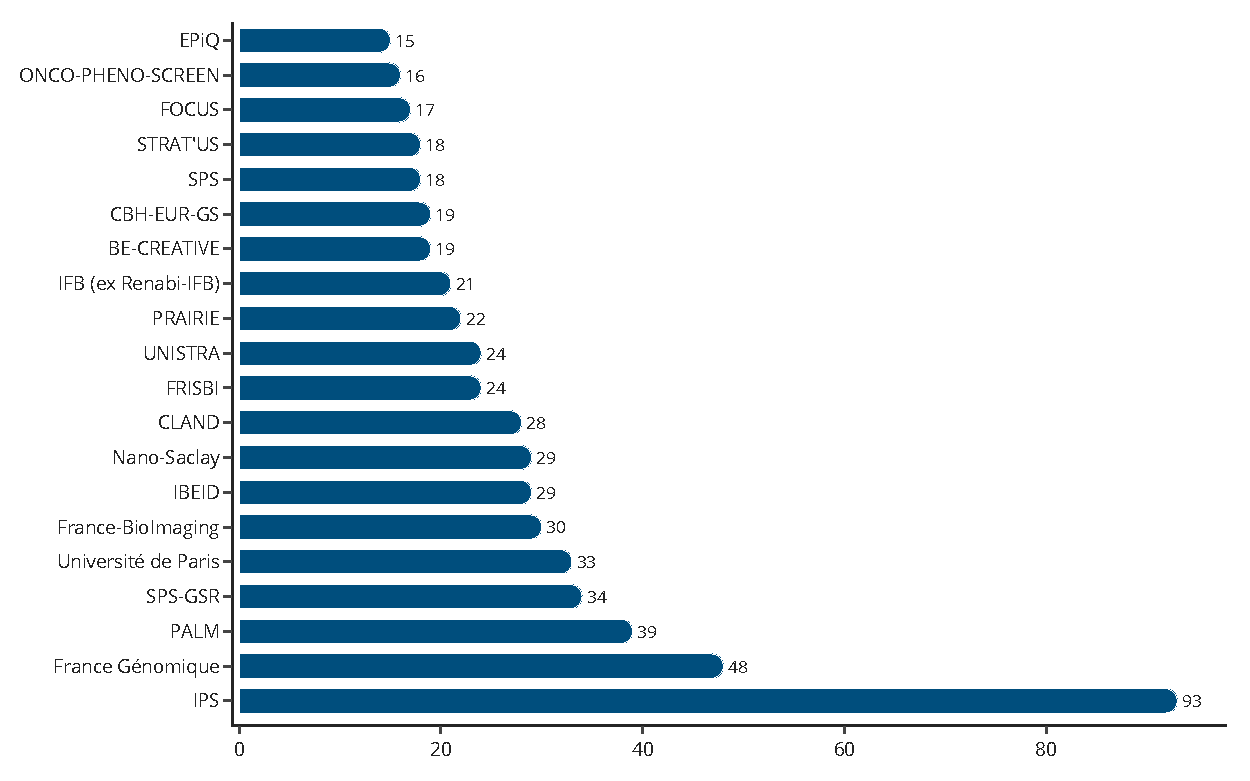
\includegraphics[width=.8\textwidth]{figures/anr_projects.pdf}
  \centering
  \caption{Projets ANR}
  \label{fig_anr_projects}
\end{figure}

% Ecrire un commentaire sur les publications liées à des projets ANR ci-dessous :





% Fin des publications liées à des projets ANR

\pagebreak

\section{Données - jeux de données partagés}

% Ecrire un commentaire sur les données - jeux de données partagés ci-dessous :





% Fin des données - jeux de données partagés

\section{Logiciels partagés}

% Ecrire un commentaire sur les Logiciels partagés ci-dessous :





% Fin des Logiciels partagés

\section{Cahiers de laboratoire partagés}

% Ecrire un commentaire sur les cahiers de laboratoire partagés ci-dessous :





% Fin des cahiers de laboratoire partagés

\pagebreak

\section{Les atouts du Laboratoire dans son engagement pour la science ouverte}

% Ecrire un commentaire sur les atouts du Laboratoire dans son engagement pour la science ouverte ci-dessous :





% Fin des atouts du Laboratoire dans son engagement pour la science ouverte 


\section{Préconisations, pour aller plus loin}

% Ecrire un commentaire sur les préconisations, pour aller plus loin ci-dessous :





% Fin des préconisations, pour aller plus loin

\vfill

\paragraph{Rappel :} la loi pour la République Numérique permet aux auteurs travaillant dans une institution publique en France depuis 2016, de partager le postprint sur HAL, avec un embargo de 6 mois pour les disciplines STM et 1 an pour les SHS.

Des formations, des accompagnements peuvent être proposées par votre référent recherche pour guider les chercheurs. 




\makelastpagereport
 
\end{document}
